\section{Study of data from K2}
\protect\label{section:k2data}

Data from K2 showed some intervals strongly affected by frequent flaring events,
however there were quiescent periods during which a regular cyclic pattern could
be observed, for example as seem in Fig. \ref{fig:k2lcurve}. This can be used to
generate a very clear periodogram as shown in Fig. \ref{fig:k2pgram}. A
phase-folded curve is shown in Fig. \ref{fig:k2pfold}.

\begin{figure}[!htbp]
\begin{center}
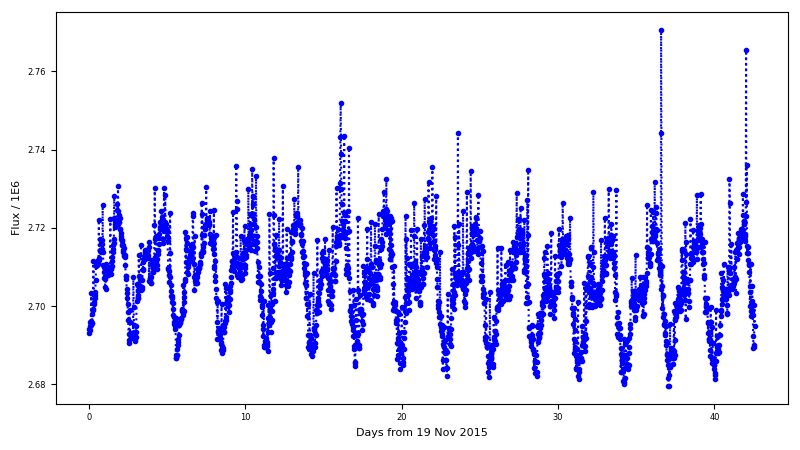
\includegraphics[scale=0.40]{k2/images/k2lcurve.png} \\
\vspace{-.5cm}
\end{center}   
\caption{Data for {\ross} taken from the archive of K2 data on MAST for 10
October 2015 onward, omitting the first 40 days, which were affected by
flares.}\protect\label{fig:k2lcurve}
\end{figure}

\begin{figure}[!htbp]
\begin{center}
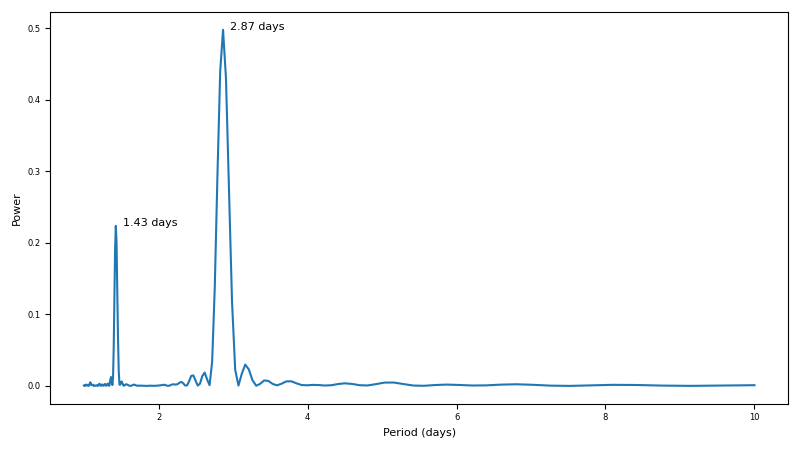
\includegraphics[scale=0.40]{k2/images/k2_pg.png} \\
\vspace{-.5cm}
\end{center}   
\caption{Periodogram taken from the data displayed in Fig.
\ref{fig:k2lcurve}}\protect\label{fig:k2pgram}
\end{figure}

\begin{figure}[!htbp]
\begin{center}
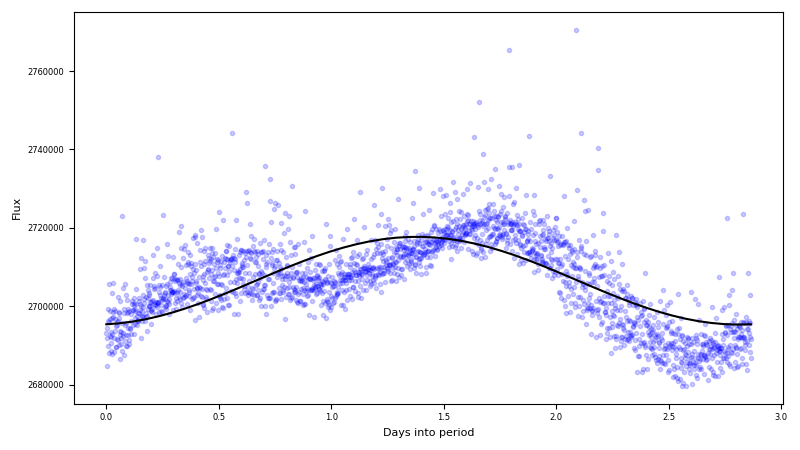
\includegraphics[scale=0.40]{k2/images/k2_pfold.png} \\
\vspace{-.5cm}
\end{center}   
\caption{Phase-folded light curve of the data shown in Fig. \ref{fig:k2lcurve}
using the peak period displayed in Fig. \ref{fig:k2pgram}.The black line marks
the fit of the peak period.}\protect\label{fig:k2pfold}
\end{figure}